%\subsection{Efficiency and Pruning Scheme Evaluation}
\begin{figure}[t]
	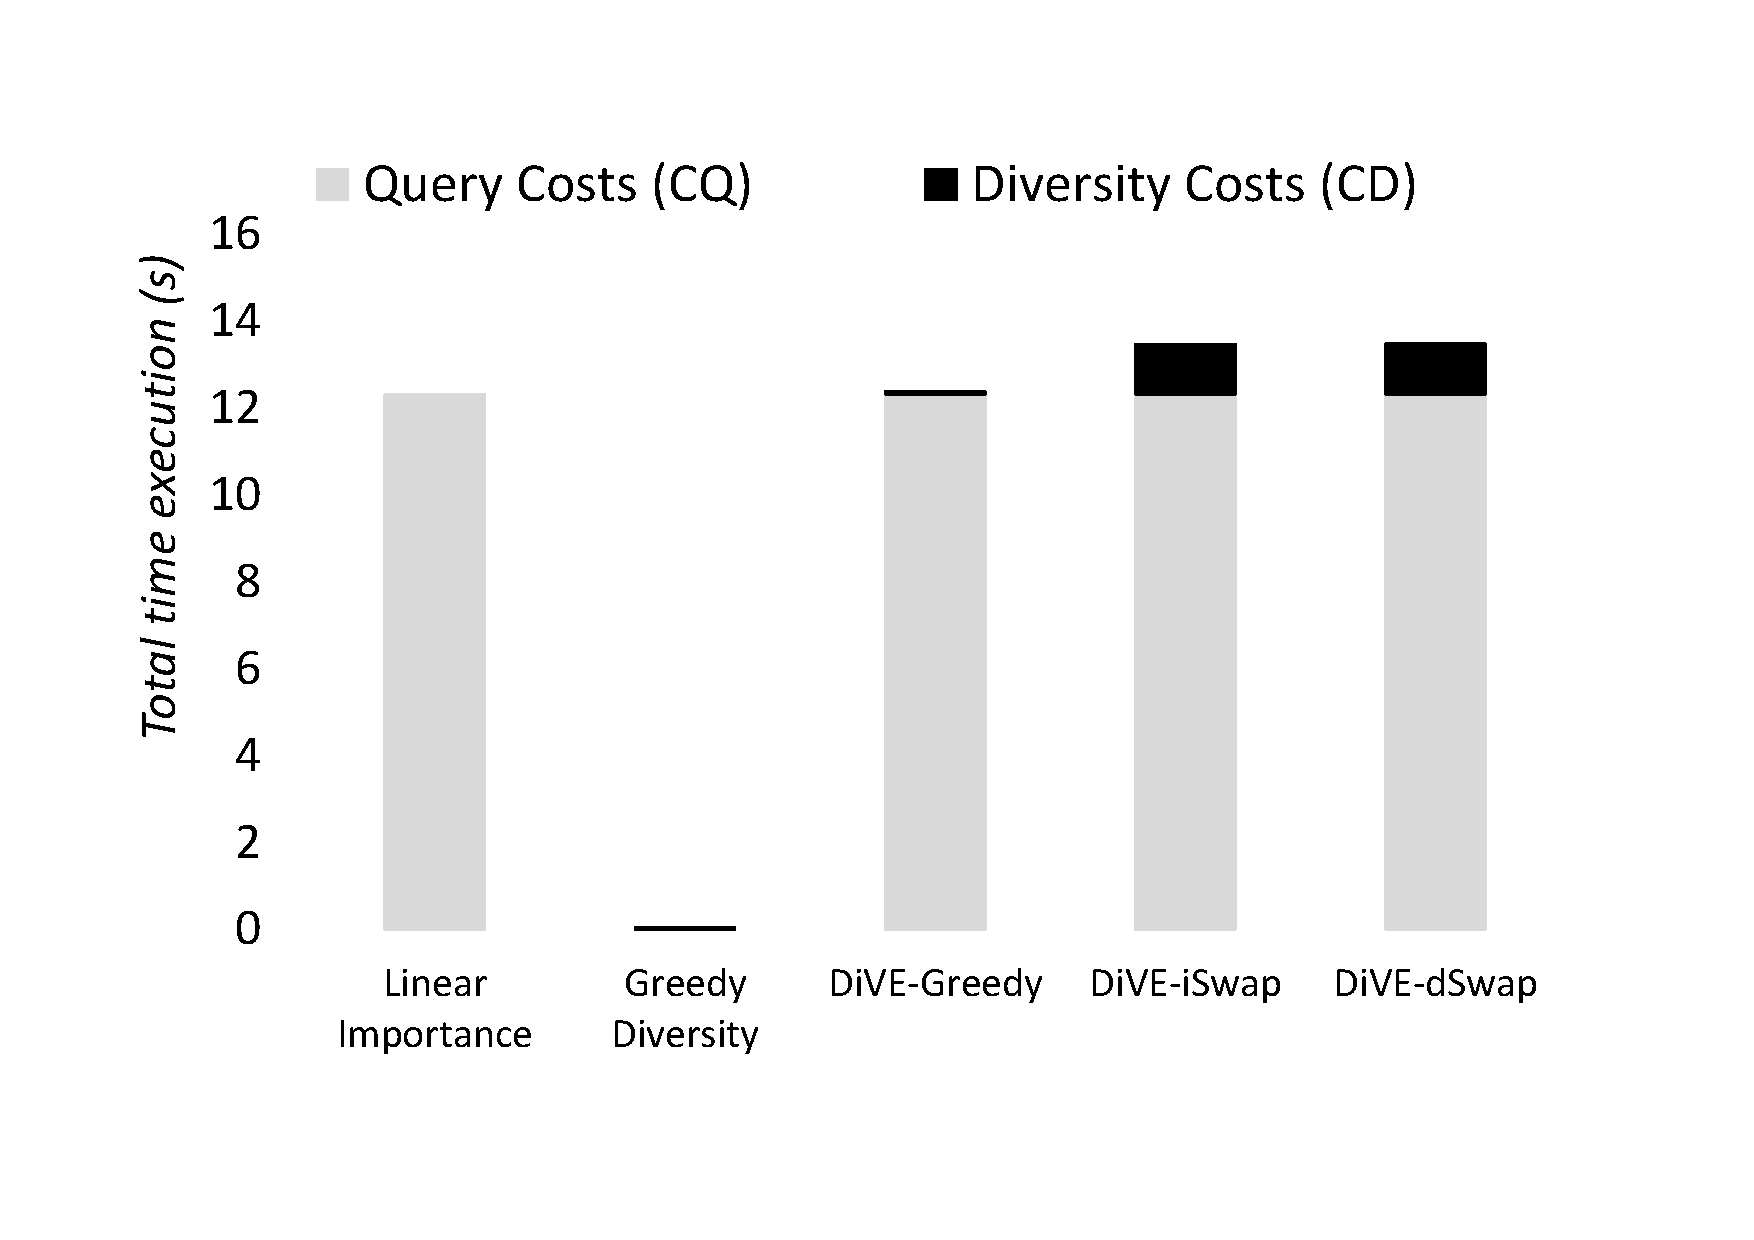
\includegraphics[width=2.6in]{figures/results/flight_costs}
		\vspace{-15pt}
	\caption{Cost Analysis of DiVE, k =5, $\lambda = 0.5$}
	\label{fig:cost_flights}
		\vspace{-5pt}
\end{figure}
% Efficiency and Pruning Scheme%

% Overall execution time / Overall costs to run all schemes%

{\noindent{\bf Execution time evaluation}}
In this experiment we measure the cost of {\em DiVE} in terms of execution time. Figure \ref{fig:cost_flights} plots the execution time for Flights dataset with $k = 5$ and $\lambda = 0.5$. The total execution time is split into the query execution time $C_Q$ and the diversification cost $C_D$. It is clear from Figure \ref{fig:cost_flights} that the total execution time $C_T$ is dominated by the cost of generating the views $C_Q$. Hence, the minimum cost is incurred by the Greedy-Diversity method which only computes diversity. For all other methods, the $C_Q$ component of the execution time is same as all views are generated only once. However, the cost of diversification $C_D$ is slightly higher for DiVE-iSwap and DiVE-dSwap as compared to the DiVE-Greedy due the higher number of iterations. 





%\subsubsection{Static-Pruning scheme performance}


% Impact of lambda (parameter to tradeoff between importance and diversity) to the pruned queries, running on Heart disease dataset %
%

\begin{figure}[t]
	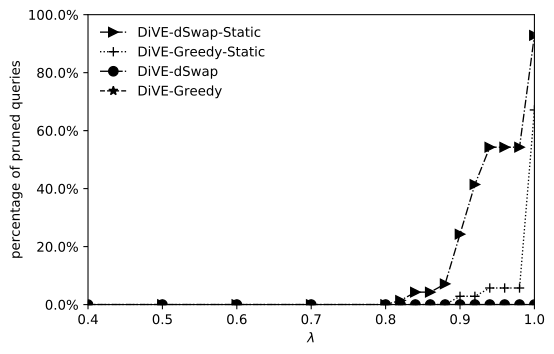
\includegraphics[width=2.6in]{figures/results/no_pruning_vs_static}
			\vspace{-15pt}
	\caption{Impact of Static pruning}%, k = 5}
	\label{fig:impact_lambda_to_PI_sampling_greedy_pruning}
		\vspace{-6pt}
\end{figure}


{\noindent{\bf Impact of static Pruning}}
In this experiment we present the performance of our proposed pruning techniques in terms of the number of pruned queries required to generate the views. The higher number of pruned queries result in the higher cost savings in the total query execution time. Figure \ref{fig:impact_lambda_to_PI_sampling_greedy_pruning} shows the performance of our static pruning technique using the maximum value of importance score $I_u$. In this and next experiments, DiVE-iSwap is not evaluated as it executes all the view queries for the initial set selection and any pruning afterwards is not possible. Moreover, due to space limit, we use only the heart disease dataset in the next experiments.

For both schemes DiVE-Greedy-Static and DiVE-dSwap-Static, since the $I_u$ value can be far from the actual importance scores of individual views, the percentage of pruned queries is $0$ for lower values of $\lambda$. Only for $\lambda$ close to $0.9$ some queries get pruned. DiVE-dSwap-Static  is able to prune higher number of queries than DiVE-Greedy-Static. At $\lambda=1$, DiVE-dSwap-Static prunes $80\%$ queries while DiVE-Greedy-Static prunes almost $65\%$ queries. 

%This is because for $\lambda = 1$ the weight of importance score is $0$ in the hybrid objective function and the overall value of $F\left(S\right)$ is determined by the diversity score only.

\begin{figure}[t]
	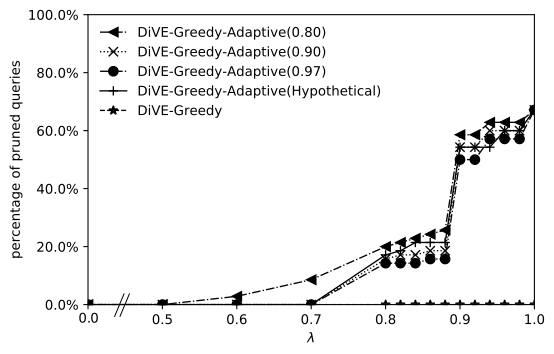
\includegraphics[width=2.6in]{figures/results/pruning_performance_greedy_adaptive}
			\vspace{-15pt}
	\caption{DiVE-Greedy with Adaptive Pruning}%, k = 5, $\lambda = 0.5$}
	\label{fig:pruning_performance_greedy}
		\vspace{-6pt}
\end{figure}

\begin{figure}[t]
	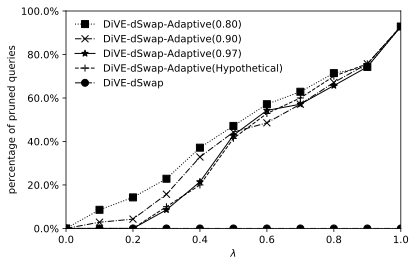
\includegraphics[width=2.6in]{figures/results/pruning_performance_dswap_adaptive}
				\vspace{-15pt}
	\caption{DiVE-dSwap with Adaptive Pruning}%, k = 5, $\lambda = 0.5$}
	\label{fig:impact_lambda_to_PI_sampling_swapd_pruning}
	\vspace{-6pt}
\end{figure}



{\noindent{\bf Impact of Adaptive Pruning}}
In this experiment we analyze the performance of adaptive pruning technique under different values of $\lambda$ and prediction interval $PI$. As shown in Figure \ref{fig:pruning_performance_greedy}, DiVE-Greedy-Adaptive is able to prune queries even for lower values of $\lambda$. The number of queries pruned increase significantly for higher values of $\lambda$. In comparison to the static pruning as shown in Figure \ref{fig:impact_lambda_to_PI_sampling_greedy_pruning}, with adaptive pruning DiVE-Greedy is able to prune almost $20\%$ more queries at $\lambda = 0.8$. Figure \ref{fig:impact_lambda_to_PI_sampling_swapd_pruning} shows the performance of DiVE-dSwap-Adaptive with different values of $ PI $. In comparison to DivE-Greedy-Adaptive, the number of pruned queries by DivE-dSwap-Adaptive are much higher for all values of $\lambda$. The interesting observation is the fact that DiVE-dSwap-Adative is able to prune $15\%$ queries for $\lambda$ values as low as $0.2$. For higher values of $\lambda$ the percentage of pruned queries is between $60\%$ and $90\%$. Similar to DiVE-Greedy-Adaptive, highest number of queries are pruned for $PI=0.8$. 
	
	%The performance declines slightly as we increase $PI$ to $0.97$. This is because when the sample size is large, many queries are already executed and the margin of cost savings by pruning the remaining queries is small.
%\end{itemize}

\begin{figure}[t]
	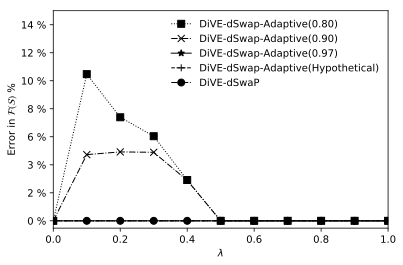
\includegraphics[width=2.6in]{figures/results/error_f_s}
				\vspace{-15pt}
	\caption{Impact of Adaptive pruning on $F(S)$}
	\label{fig:pruning_performance_swapd}
\end{figure}

Further we evaluate the effectiveness of methods with adaptive pruning in terms of the $F\left(S\right)$ values. 
%Although, adaptive pruning is based on approximation of the actual importance score bounds, still the loss in the $F\left(S\right)$ values of the computed set of views is very small. 
Figure \ref{fig:pruning_performance_swapd} shows the loss in $F\left(S\right)$ in comparison to the $F\left(S\right)$ values achieved by Hypothetical methods. The loss for both DiVE-Greedy-Adaptive and DiVE-dSwap-Adaptive is $0\%$ for $PI=0.97$, With a larger sample size the accuracy of approximated importance score is higher. For a smaller sample size of $PI=0.80$ there is 0\% loss while $\lambda = 0$ because at the moment there are no pruned queries. However, there is a maximum loss of $10\%$ at $\lambda= 0.1$. The loss in $F\left(S\right)$ values decrease as $\lambda$ increases as the impact of importance score becomes smaller in the hybrid objective function. Meanwhile, starting $\lambda \geq 0.5$ the loss is 0\%.

% it can be confirmed in Figure \ref{fig:impact_lambda_to_PI_sampling_swapd_pruning} that shows the performance of DiVE-dSwap-Adaptive($0.80$) close to DiVE-dSwap-Adaptive($0.97$) and DiVE-dSwap-Adaptive(Hypothetical) which there is no loss for both of them.

\eat{
% The impact of query load to the pruning performance %
{\noindent{\bf The impact of query subset on pruning}}
The pruning power of our algorithms is effected by the maximum importance score views generated over a data subset $D_Q$ in comparison to the reference subset $D_R$. If the highest importance score of any view generated over $D_Q$ is far less than the upper bound of $\sqrt{2}$ (Sec. ~\ref{subsec:problem_definition}), then only few queries will be pruned. 
%
%Similarly, for adaptive pruning technique higher or lower importance scores of views will effect the number of pruned queries. 
%
Thus, for this experiment, we created three different clusters of heart disease subsets. And categorized them as low, medium and high. Where low dataset is the subset with low values of importance score (i.e., {\tt low importance query load}) and high is the subset with higher values of importance score (i.e., {\tt high importance query load}). We run experiments using those two type of query load and compared the performance of pruning methods in terms of number of queries pruned. The $ PI $ value is set to default value of $0.97$. It can be seen in Figure \ref{fig:low_vs_high} that both DiVE-Greedy-Adaptive and DiVE-dSwap-Adaptive perform better on low importance query load. For high importance query load less number of queries are pruned. This shows that the characteristic of the query subset $D_Q$ has an impact on the efficiency of the pruning methods.


\begin{figure}[t]
	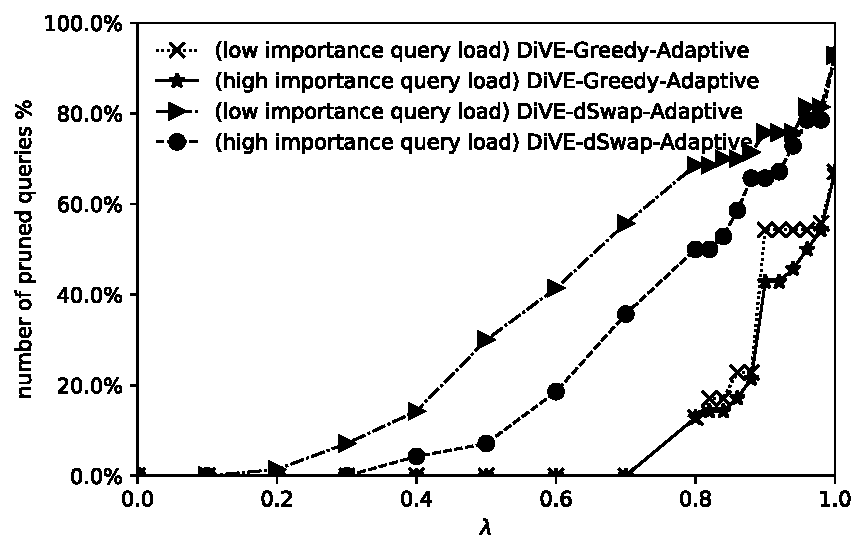
\includegraphics[ width=2.6in]{figures/results/low_vs_high_new}
			\vspace{-15pt}
	\caption{Impact of Query Subset}
	\label{fig:low_vs_high}
\end{figure}
}
%
%
%\eat{
%	\textbf{\textit{The total time to run DiVE schemes}}. In order to start analyzing the efficiency, we need to know the main issue in term of costs. Figure \ref{fig:cost_flights} shows the example of exactly time that needed to run schemes on flights dataset. It shows Greedy-Diversity which only considering diversity and no query executions, it has very low costs. Meanwhile, Linear-Importance and \textit{DiVE-Greedy} seems in the same line but that was not exactly same. The total of diversity computations $ C_D $ of \textit{DiVE-Greedy} is very low, the total costs of \textit{DiVE-Greedy} is dominated by query costs $ C_Q $. Due to of this reason, the total execution time of \textit{DiVE-Greedy} closes to Linear-Importance. Those are the proof that the total costs of all schemes execpt Greedy-Diversity are dominated by query cost $ C_Q $. }
%
%\eat{
%	Due to the page limitation, all our experiments in three real dataset cannot be showed. Hence, for the next sections, we use heart disease dataset as our focus observation. 
%	% Static Pruning Scheme Performance%
%}
%
%\eat{
%	\textbf{\textit{Impact of $\lambda$ to the pruned queries of \textit{DiVE-Greedy} scheme}}. In this work, we proposed two kind of pruning schemes, that are using estimated static value of maximum value of the importance score $maxI$ and using adaptive maximum value of importance score. 
%	
%	The first our pruning scheme is using static value $maxI$. To check the performance of our pruning scheme, we run it to all real datasets using different value of $ \lambda $. We analyze the result by comparing the result of schemes with pruning enable on it and the schemes without pruning enable on it. The example result which running on heart disease dataset is shown in Figure \ref{fig:pruning_performance_greedy} . The static pruning scheme only able to prune queries while the value of $\lambda$ is high, closes to 0.9. As we expected, it is because the value of $maxI$ that too far from the real value of importance score. 
%	
%	%\subsubsection{Adaptive scheme performance}
%	To overcome the flaw in static pruning scheme, we also proposed adaptive pruning scheme which used dynamic value of the maximum importance score $maxI$. In order to get $maxI$ as close as possible to the real value of importance in the dataset, we applied sampling method. By using adaptive pruning, users also able to change the confidence and the margine error to tradeoff between time and precision. 
%	
%	% Impact of lambda to the pruned queries for adaptive pruning scheme %
%	
%	\textbf{\textit{Impact of $\lambda$ to the pruned queries of \textit{DiVE-dSwap} scheme}}. If static pruning scheme only able to prune queries while $\lambda$ closes to 0.9 and higher, in this section, we shows the adaptive pruning performance. Figure \ref{fig:pruning_performance_swapd} shows the performance of adaptive pruning scheme by using different value of $\lambda$. It shows the impact of $\lambda$ to the percentage of pruned queries. The adaptive pruning schemes especially \textit{DiVE-dSwap-Adaptive} is able to prune queries significantly, pruning start while $\lambda$ closes to 0.2 and by increasing the $\lambda$, more queries can be pruned.
%}